\documentclass[main.tex]{subfiles}
\begin{document}
This is under construction
...

...

Python 程序 xxx 生成希腊的字母如下:

Α Β Γ Δ Ε Ζ Η Θ Ι Κ Λ Μ Ν Ξ Ο Π Ρ Σ Τ Υ Φ Χ Ψ Ω

α β γ δ ε ζ η θ ι κ λ μ ν ξ ο π ρ ς σ τ υ φ χ ψ ω

从 Unicode 表中 Python 程序 xxx 生成部分常用数学运算速度符号如果下:
∀ ∁ ∂ ∃ ∄ ∅ ∆ ∇ ∈ ∉ ∊ ∋ ∌ ∍ ∎ ∏ ∐ ∑ − ∓ ∔ ∕ ∖ ∗ ∘ ∙ √ ∛ ∜ ∝ ∞ ∟ ∠ ∡ ∢ ∣ ∤ ∥ ∦ ∧ ∨ ∩ ∪ ∫ ∬ ∭ ∮ ∯ ∰ ∱ ∲ ∳ ∴ ∵ ∶ ∷ ∸ ∹ ∺ ∻ ∼ ∽ ∾ ∿ ≀ ≁ ≂ ≃ ≄ ≅ ≆ ≇ ≈ ≉ ≊ ≋ ≌ ≍ ≎ ≏ ≐ ≑ ≒ ≓ ≔ ≕ ≖ ≗ ≘ ≙ ≚ ≛ ≜ ≝ ≞ ≟ ≠ ≡ ≢ ≣ ≤ ≥ ≦ ≧ ≨ ≩ ≪ ≫ ≬ ≭ ≮ ≯ ≰ ≱ ≲ ≳ ≴ ≵ ≶ ≷ ≸ ≹ ≺ ≻ ≼ ≽ ≾ ≿ ⊀ ⊁ ⊂ ⊃ ⊄ ⊅ ⊆ ⊇ ⊈ ⊉ ⊊ ⊋ ⊌ ⊍ ⊎ ⊏ ⊐ ⊑ ⊒ ⊓ ⊔ ⊕ ⊖ ⊗ ⊘ ⊙ ⊚ ⊛ ⊜ ⊝ ⊞ ⊟ ⊠ ⊡ ⊢ ⊣ ⊤ ⊥ ⊦ ⊧ ⊨ ⊩ ⊪ ⊫ ⊬ ⊭ ⊮ ⊯ ⊰ ⊱ ⊲ ⊳ ⊴ ⊵ ⊶ ⊷ ⊸ ⊹ ⊺ ⊻ ⊼ ⊽ ⊾ ⊿ ⋀ ⋁ ⋂ ⋃ ⋄ ⋅ ⋆ ⋇ ⋈ ⋉ ⋊ ⋋ ⋌ ⋍ ⋎ ⋏ ⋐ ⋑ ⋒ ⋓ ⋔ ⋕ ⋖ ⋗ ⋘ ⋙ ⋚ ⋛ ⋜ ⋝ ⋞ ⋟ ⋠ ⋡ ⋢ ⋣ ⋤ ⋥ ⋦ ⋧ ⋨ ⋩ ⋪ ⋫ ⋬ ⋭ ⋮ ⋯ ⋰ ⋱ ⋲ ⋳ ⋴ ⋵ ⋶ ⋷ ⋸ ⋹ ⋺ ⋻ ⋼ ⋽ ⋾ ⋿

\begin{figure}
	\centering
	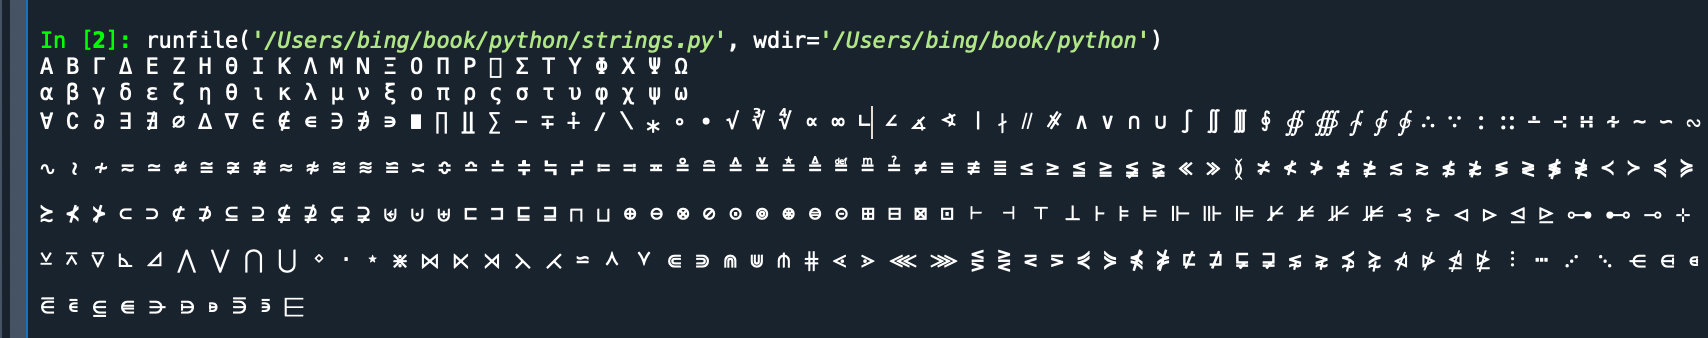
\includegraphics{images/greek_math_symbols.png}
\end{figure}


dkalfadsf

\newpage
\end{document} 